\documentclass[a4paper,5pt]{amsbook}
%%%%%%%%%%%%%%%%%%%%%%%%%%%%%%%%%%%%%%%%%%%%%%%%%%%%%%%%%%%%%%%%%%%%%

\usepackage{booktabs}
\usepackage{graphicx}
\usepackage{multicol}
\usepackage{textcomp}
\usepackage{systeme}
\usepackage{amssymb}
\usepackage{amsmath}
\usepackage{subcaption}
\usepackage[inline]{enumitem}

%%%%%%%%%%%%%%%%%%%%%%%%%%%%%%%%%%%%%%%%%%%%%%%%%%%%%%%%%%%%%%

\newcommand{\sen}{\,\mbox{sen}\,}
\newcommand{\tg}{\,\mbox{tg}\,}
\newcommand{\cosec}{\,\mbox{cosec}\,}
\newcommand{\cotg}{\,\mbox{cotg}\,}
\newcommand{\tr}{\,\mbox{tr}\,}
\newcommand{\ds}{\displaystyle}

%%%%%%%%%%%%%%%%%%%%%%%%%%%%%%%%%%%%%%%%%%%%%%%%%%%%%%%%%%%%%%%%%%%%%%%%

\setlength{\textwidth}{16cm} %\setlength{\topmargin}{-1.3cm}
\setlength{\textheight}{26cm}
\setlength{\leftmargin}{1.2cm} \setlength{\rightmargin}{1.2cm}
\setlength{\oddsidemargin}{0cm}\setlength{\evensidemargin}{0cm}
\setlength{\topmargin}{-1cm}

%%%%%%%%%%%%%%%%%%%%%%%%%%%%%%%%%%%%%%%%%%%%%%%%%%%%%%%%%%%%%%%%%%%%%%%%

% \renewcommand{\baselinestretch}{1.6}
% \renewcommand{\thefootnote}{\fnsymbol{footnote}}
% \renewcommand{\theequation}{\thesection.\arabic{equation}}
% \setlength{\voffset}{-50pt}
% \numberwithin{equation}{chapter}

%%%%%%%%%%%%%%%%%%%%%%%%%%%%%%%%%%%%%%%%%%%%%%%%%%%%%%%%%%%%%%%%%%%%%%%

\begin{document}
\thispagestyle{empty}
\pagestyle{empty}
\begin{minipage}[h]{0.14\textwidth}
	
\includegraphics[scale=0.24]{../../ufgd.png}
\end{minipage}
\begin{minipage}[h]{\textwidth}
\begin{tabular}{c}
{{\bf UNIVERSIDADE FEDERAL DA GRANDE DOURADOS}}\\
{{\bf Geometria --- Lista 2}}\\
{{\bf Prof.\ Adriano Barbosa}}\\
\end{tabular}
\vspace{-0.45cm}
%
\end{minipage}

%------------------------

\vspace{1cm}
%%%%%%%%%%%%%%%%%%%%%%%%%%%%%%%%   formulario  inicio  %%%%%%%%%%%%%%%%%%%%%%%%%%%%%%%%
\begin{enumerate}
    \item Seja $D$ um ponto interior de um tri\^angulo equil\'atero $ABC$ de lado
        $\ell$ tal que $\overline{AD} = 7$, $\overline{BD} = 8$ e
        $\overline{CD} = 5$. Considere um ponto $E$ no exterior do tri\^angulo
        $ABC$, conforme a figura, tal que o \^angulo $D\hat{C}E = 60^\circ$ e
        $\overline{CD} = \overline{CE}$.
        \begin{enumerate}
            \vspace{0.3cm}
            \item Mostre que os tri\^angulos $ACE$ e $BCD$ s\~ao congruentes.
            \vspace{0.3cm}
            \item Determine os comprimentos dos segmentos $AE$ e $DE$.
            \vspace{0.3cm}
            \item Encontre a medida do \^angulo $A\hat{E}D$.
            \vspace{0.3cm}
            \item Encontre o valor de $\ell$.
        \end{enumerate}
        \begin{figure}[!h]
            \centering
            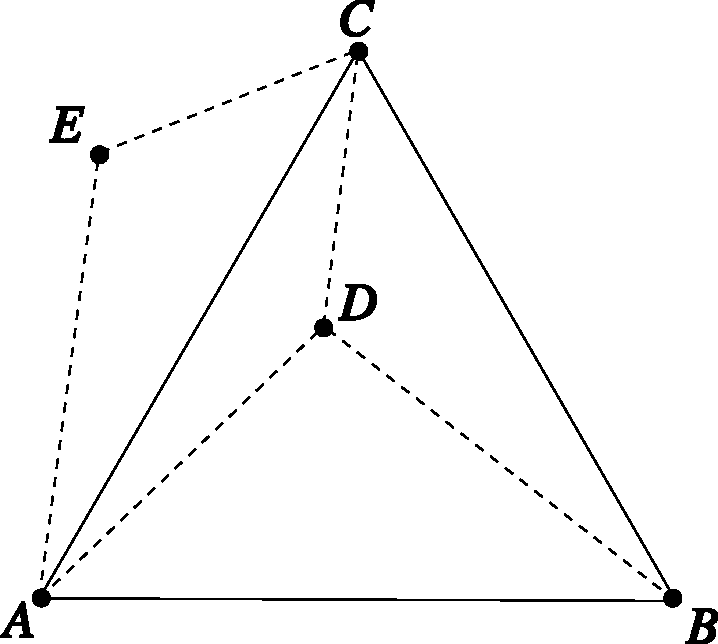
\includegraphics[width=0.2\textwidth]{fig02-1.pdf}
        \end{figure}

    \vspace{0.5cm}
    \item No cilindro circular reto da figura, o raio da base mede 3cm e a
        altura mede 9cm. Sabe-se ainda que o segmento $AB$ \'e perpendicular \`as
        bases e que o comprimento do menor arco $AC$ \'e $2\pi$cm.
        \begin{enumerate}
            \vspace{0.3cm}
            \item Determine a medida do segmento $BC$.
            \vspace{0.3cm}
            \item Determine o \^angulo $A\hat{B}C$.
        \end{enumerate}
        \begin{figure}[!h]
            \centering
            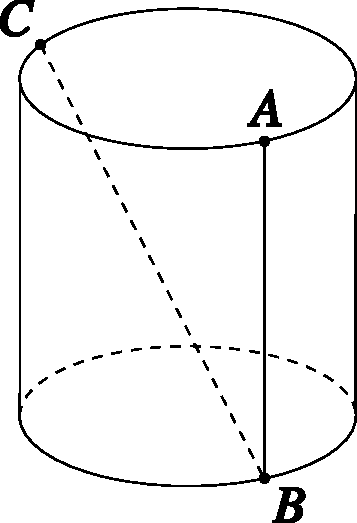
\includegraphics[width=0.15\textwidth]{fig02-2.pdf}
        \end{figure}

    \item O cubo $ABCDEFGH$ da figura tem aresta igual a $a$. Os pontos $M$,
        $N$ e $P$ s\~ao os centros das faces $AFED$, $DEHC$ e $CBGH$,
        respectivamente
        \begin{enumerate}
            \vspace{0.3cm}
            \item Determine o \^angulo entre as faces $MPA$ e $MPN$ do tetraedro
                $AMPN$.
            \vspace{0.3cm}
            \item Determine o volume do tetraedro $AMPN$.
        \end{enumerate}
        \begin{figure}[!h]
            \centering
            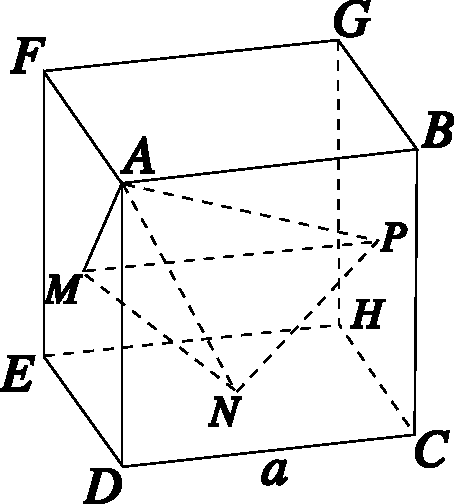
\includegraphics[width=0.25\textwidth]{fig02-3.pdf}
        \end{figure}

    \vspace{0.5cm}
    \item Dado um tri\^angulo $ABC$, sejam $M$ o ponto m\'edio do segmento $BC$ e
        $\Gamma$ a circunfer\^encia tal que o segmento $AB$ \'e um di\^ametro. Prove
        que $\overline{AB} = \overline{AC}$ se, e somente se, $M$ pertence \`a
        circunfer\^encia $\Gamma$.

    \vspace{0.5cm}
    \item Um segmento que tem um v\'ertice de um tri\^angulo como uma das suas
        extremidades e a outra extremidade sobre o lado oposto a esse v\'ertice \'e
        chamado de \textit{ceviana interna} do tri\^angulo. O Teorema de Ceva
        afirma que, em um tri\^angulo $ABC$, as cevianas internas $AA'$, $BB'$ e
        $CC'$ se intersectam em um mesmo ponto se, e somente se,
        \[\frac{\overline{BA'}}{\overline{A'C}} \cdot
        \frac{\overline{CB'}}{\overline{B'A}} \cdot
        \frac{\overline{AC'}}{\overline{C'B}} = 1.\]
        Prove, utilizando o Teorema de Ceva, que em um tri\^angulo $ABC$:
        \begin{enumerate}
            \vspace{0.3cm}
            \item As tr\^es medianas de um tri\^angulo concorrem em um mesmo ponto.
            \vspace{0.3cm}
            \item As tr\^es bissetrizes internas de um tri\^angulo concorrem em um
                mesmo ponto.
        \end{enumerate}
        \begin{figure}[!h]
            \centering
            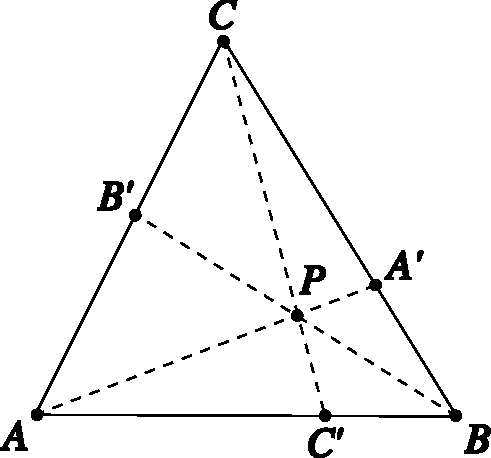
\includegraphics[width=0.25\textwidth]{fig02-4.pdf}
        \end{figure}
\end{enumerate}

\end{document}
